\section{Datenbanken}
Weltweit wurden im Jahr 2022 Daten im Umfang von 103.66 Zettabyte erfasst. Diese Zahl wird sich laut Statistik \ref{fig:DatenvolumenStatistik} bis zum Jahr 2026 verdoppelt haben. Angesicht dieser Zahlen, sind Datenbanken aus der heutigen Zeit nicht weg zu denken. Sie bieten eine Möglichkeit, große Mengen an Daten Strukturiert abzuspeichern und anschließend auszuwerten.\\
Hierbei werden Datenbanken Grundsätzlich in Zwei Kategorien unterteilt. Relatione Datenbank und "Nicht relatione Datenbanken". Unterschiede der Datenbankarten machen sich in der Sprache zum Auswerten der DB, ihrer Skalierbarkeit, der Struktur, der Eigenschaften und der Unterstützung durch die Comunity bemerkbar. 
\begin{center}
    \begin{figure}[h]
     \centering
     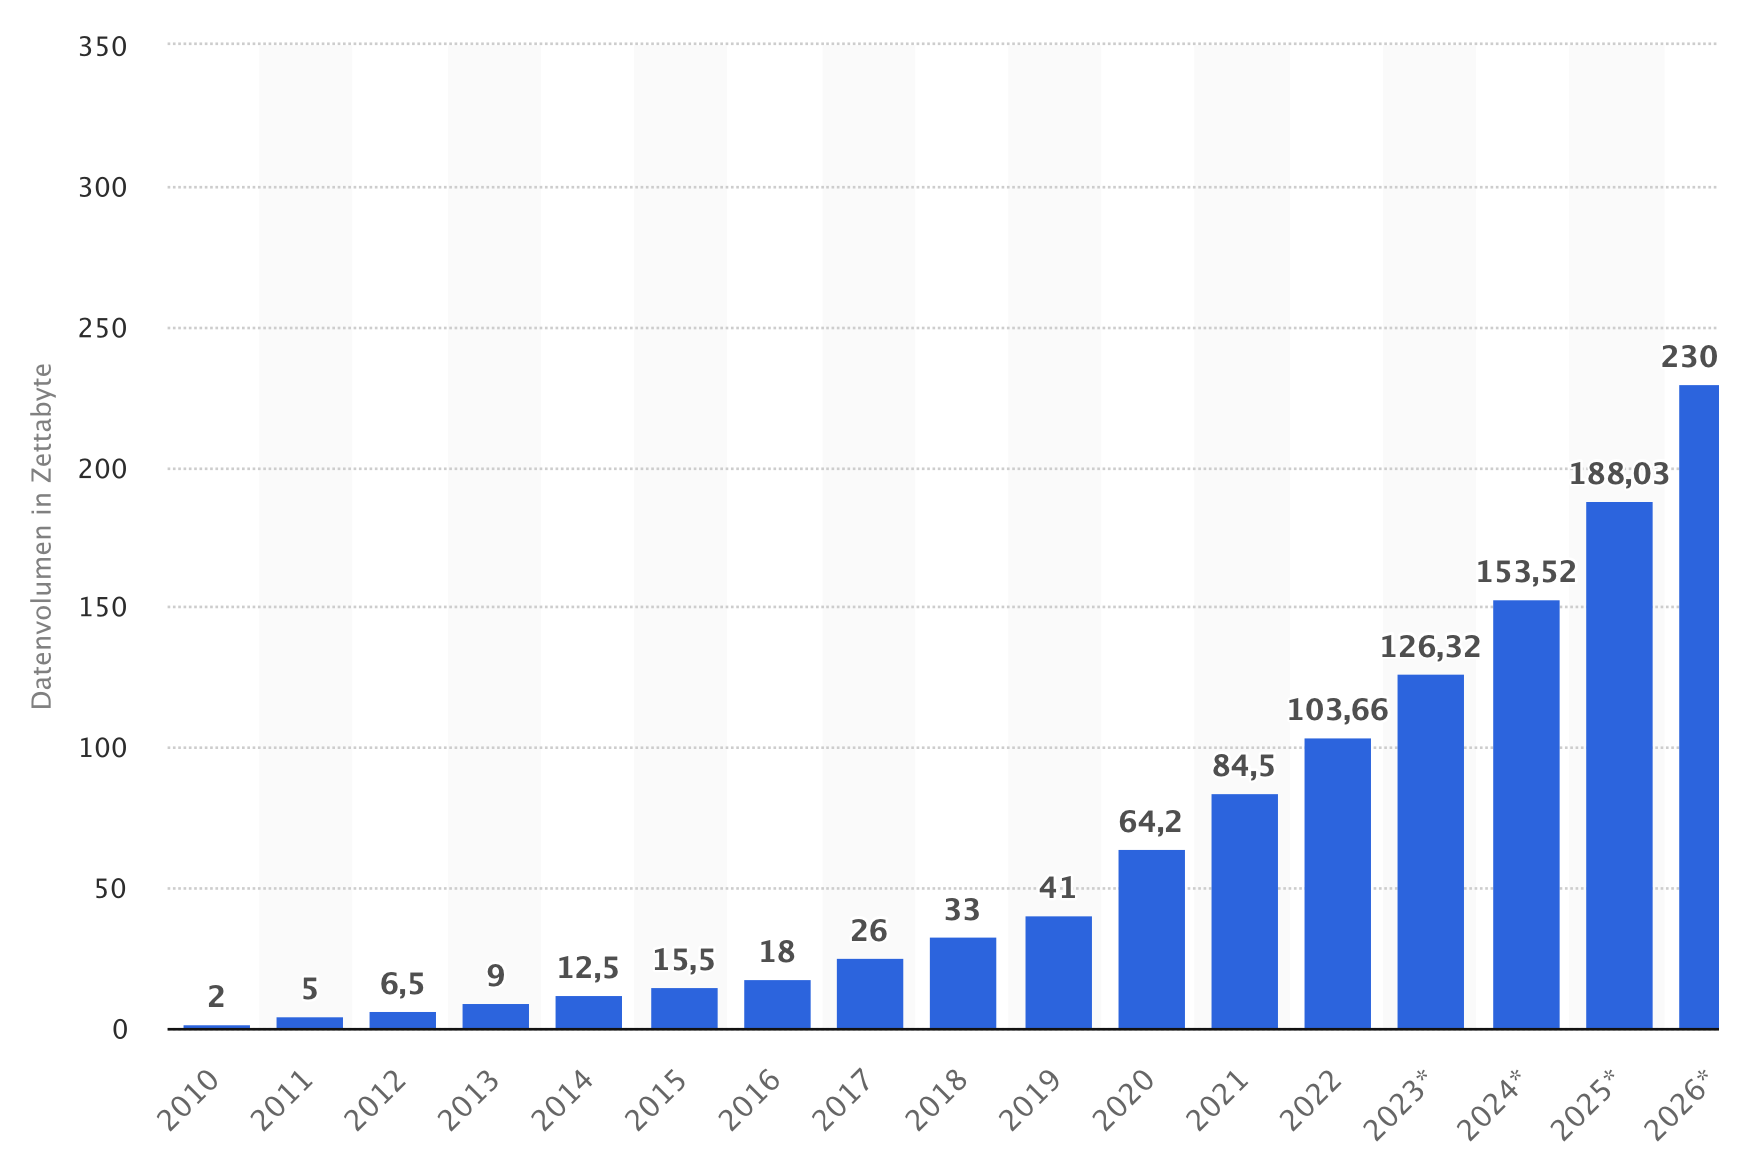
\includegraphics[width=1\linewidth]{DatenvolumenStatistik}
     \caption{Volumen der weltweit generierten Daten bis 2027 \cite{Datenmengen}}
    \label{fig:DatenvolumenStatistik}
    \end{figure}
\end{center}
\subsection{SQL - Structured Query Language}
IBM-Forscher Edgar F. Codd definierte 1969 ein Datenbankmodell für Relationale Datenbanken. Auf grundlagen seiner Forschung began, in den folgenden Jahren, die entwicklung der Sprache \ac{sequel}. Codds Modell für bassiert auf der zuordnung von Schlüsseln. Nach einigen Überarbeitungen der implementierung wurde diese anschließend in \ac{sql} umbenannt.\\
\ac{sql} ermöglicht insbesondere die Speicherung, Bearbeitung so wie eine Abfrage von Daten in einer Datenbank. Mithilfe des Prinzips der Schlüssel, können Datensätze miteinander verknüpft werden. Somit kann einem Benutzernamen bespielsweise ein echter Name, eine Telefonnummer und eine Email-Addresse zugewiesen werden.\\
Die besondere eigenschaft von \ac{sql} ist das Konzepte von Arrays. Relationale Datenbanken bestehen aus Arrays, welche sich mit Hilfe von verschiedenen Befehen erzeugen und bearbeiten. \cite{sql}\\
\ac{sql} beitet eine reihe von Befehlen, welche die Interaktion mit der Datenbank ermöglichen. Diese können Grundsätzlich in 5 Kategorien eingeteilt werden (siehe Abb. \ref{fig:SQLCommands}). Die wichtigsten Befehle sind dabei \text{INSERT}, \textit{UPDATE} und \textit{DELEAT}, mit welchen sich datensätze schreiben und bearbeiten lassen. Zudem der kommt der \textit{SELECT} Befehl, welcher das auslesen von Datensätzen ermöglicht. Um die tabellenstruktur der Datenbank zu berarbeiten kommen die Befehle \textit{CREATE} und \textit{DROP} zum einsatz. \cite{SQLCommands}\\
Natürlich bietet die Programmiersprache eine weit aus komplexere Sysntax, um datensätze sortiet auswerten zu könen. Eine vollständige dokumentation der Sprache findet sich auf der w3school webseite \cite{SQLDoku}.
\begin{center}
    \begin{figure}[h!]
     \centering
     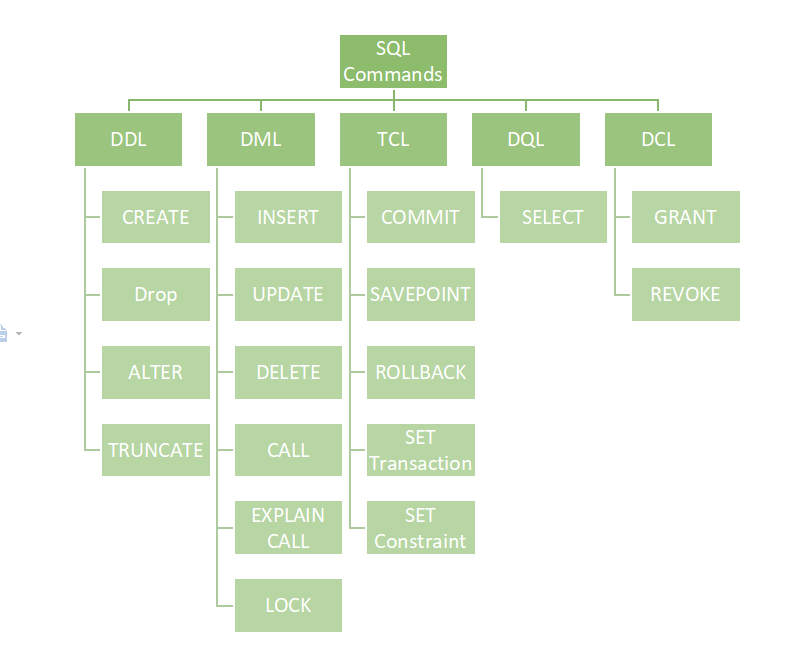
\includegraphics[width=1\linewidth]{SQLCommands}
     \caption{SQL Befehls Kategorien \cite{SQLCommands}}
    \label{fig:SQLCommands}
    \end{figure}
   \end{center}

\subsection{SQLite Embedded Datenbank}
In der Vorarbeit zu dieser Bachelorarbeit wurde bereits eine auswahl für eine Datenbank getroffen. Dabei wurde sich nach einigen vergleichen für die SQLite Embedded Datenbank Engine entschieden. \\
Diese Bietet eine zuverlässige, kleine, schnelle und vollfunktionale Datenbank Engine, welche vollständige in das Gesamtsystem integriert werden kann \cite{SQLiteHompage}. Zur implementierung der Datenbank in die anwendung wird die System.Data.SQLite Bibliothek für C\# verwendet.\\